\chapter{Background Literature}
\label{BackgroundLit}


\section{Dementia and HCI}
\label{BL:DementiaHCI}
Over the last 40 years, researchers and care practitioners have seen our understanding of dementia evolve to position and represent the person with dementia in several ways. What was once a bio-medical stance has gradually moved towards one that considers the socio-political and individual experiences of dementia \citep{bellass_broadening_2019} . In the early years of dementia research, the biomedical view, dementia was viewed through its neurodegenerative condition, emphasising the person's abilities, memory, judgement and communication. Recognising these characteristics of dementia led to an awareness of strain on care partners towards policymakers, improvements in identifying and diagnosing dementia, and the development of medication to reduce symptoms of dementia \citep{doi:10.1080/13607863.2019.1693968}. Moreover, given that there are still no known treatments to stop the progression of dementia, there has been significant work and research funding into understanding the causes of the neurodegenerative condition \citep{bature_signs_2017}.

However, several negative consequences arose from such a biomedical lens that has had significant social ramifications on people with dementia. First, the biomedical view promotes a view of 'loss of self' \citep{ryan_dementia_2009}. Early work by \cite{cohen_loss_1986} believed that people living with dementia \textit{"must eventually come to terms with…the complete loss of self"}. Views of dementia that see it as a state of deficiency, often place the person living with dementia as a passive \textit{'patient'} where the condition is looked at being treated rather than understood. If acted upon, design and research do very little to aid the agency or the need for a continued sense of purpose and belonging \citep{hampson_dementia:_2016}. Second, as dementia progresses, it often adds conflict between their surroundings as they become unfamiliar, and in turn, causes difficulties coexisting in places with others, such as a family home or a workplace \citep{langdon_making_2007}. Finally, As we live in a society that places great value on cognitive ability, many believe that people with dementia are poor at social contact, which then prohibits many from interacting with people with dementia at all \citep{killick_communication_2001}.

From the early 90's, researchers began to contest the limitations of the biomedical stance by highlighting that the quality of life of the person with dementia is determined not only by neuropathology but also by how they are perceived in society, personal history, and interactions and desires \citep{o2007personhood}. There is growing literature indicating that an approach to care that supports inclusion, recognition, trust, and the individual's personhood may delay or reduce several negative consequences that may develop with dementia. Tom Kitwood, one of the more prominent researchers to tackle the biomedical view, defined the personhood of the person with dementia as \textit{"the standing or status that is bestowed upon one human being, by others, in the context of relationship and social being"} \citep[pg.8]{kitwood1997dementia}. Instead of seeing the person with dementia by their disease, Kitwood challenged this by centring the personhood of the person with dementia by personalising care, paying attention to the individual's relationships, and maintaining decision-making by acknowledging the person's abilities. While I describe the potential limitations of personhood in the later stages of this literature review, the concept of personhood has promoted necessary changes to dementia research and practice. For instance, the approach has brought forth the sharing of people's experiences with dementia that has redefined how we speak and involve people with dementia in research. Furthermore, the focus on lived experiences, has not only demonstrated the importance of individuality in care and when working with people living with dementia but has created a cultural and positive change towards those who have recently been diagnosed with dementia and began to address 'dementia worry' \citep{kessler_dementia_2012}.

An integral part of HCI work builds on personhood approaches where design and technology advancements have moved towards improving quality of life, supporting inclusion, evoking emotion, and engagement through creativity to help foster heightening subjective wellbeing, maintaining skills, and providing social engagement. While many creatively oriented technologies have relied on the person's ability to articulate past events or configure dementia as a series of problems, as researchers have moved toward the inclusion of the voices of people living with dementia, recent HCI research has similarly begun to question how to position people with dementia in the designing of technology appropriately. With this in mind, the following subsections review dementia-HCI literature that investigates the type of technologies, design, and participatory approaches researchers use in the domain.
% Add something here making it very clear what the nxt section is. Reviewing the literature -- highlight the current state of HCI literature + potential challenges / themes that the PhD will explore

\subsection{Moving to a user-centered approach}
\label{BL:Tech}
Within HCI, early work in dementia focused on the role of assistive (or enabling) technology to support independent living for people with dementia. \cite{bharucha2009intelligent} review of assistive technology applications highlight an array of different sensors and devices built to compensate for physical and cognitive deficits of people with dementia. For instance, the authors highlight one device, in particular, GPS, to tackle the problem of 'wandering'. The term wandering derives from categorising particular 'behaviours' in people with dementia where individuals may get lost or forget where they were going. While walking is beneficial to the person with dementia, the action of 'wandering' has often been associated with potential harm and emotional stress for the person with dementia and their care partners (Robinson - balancing rights and risks). As \cite{bharucha2009intelligent} highlight, these early studies focusing on 'problems' caused by dementia, would be guided by family and professional care staff instead of people with dementia. Similarly, early work in care home architecture \citep{torrington2006has}, care processes \citep{rabins2006practical}, and creative therapy \citep{schmitt2006creative} prioritised those without dementia in the development processes with the potential of people with dementia invited in the evaluation phases of development. This has resulted in prior products and services failing to represent the desires and needs of people with dementia causing a lack of uptake and ownership of technology design \citep{gibson2019personalisation}. 

Given the overwhelming focus on technology that considers how to 'fix' challenges, researchers have introduced user-centred, participatory design methods that have brought attention to promoting personhood through the technologies we are designing. For instance, \cite{robinson2009keeping} ran a series of user-centred design sessions with people with dementia and their carers to design and develop a set of prototypes to facilitate independence for the person with dementia and centre the voices of people with dementia in the design process. The authors' findings highlight opportunities for involving people with dementia in technology's design and curation stages. The technology customisation was well received and necessary to be tailored to the person with dementia's assistive needs. However, while this work stresses that there is no one-size-fits-all approach when designing assistive technologies, researchers need to consider how we may design mass customisation techniques to deliver commercial personalised devices. Furthermore, \cite{robinson2009keeping} remark that adoption will require the support of user-friendly interfaces for carers to ensure the person with dementia use the assistive technology. 

\cite{wallace_enabling_2012-1wallace_design-led_2013} extends the user-centred approach by turning to a more experiential and relational approach known as experience-centred design (ECD). Through this approach, ECD focuses on \textit{"an understanding of individuals, their concerns, desires, aspirations, values, and experiences"} \citep{morrissey_value_2017} constructed by dialogue, storytelling, and reflection. In Wallace's paper - A Design-led Inquiry into Personhood in Dementia \citep{wallace_design-led_2013}, the author's works closely with a married couple (John and Gillian), where the wife had recently been diagnosed with dementia, to design pieces of digital jewellery to support Gillian's personhood. To involve and empathically engage the couple in the design process of the jewellery, the study was carried out as a piece of research through design (RTD). RTD is a way of doing research, which is the practice of design used to address wicked problems that entail a sense of complexity and have no current solution. The approach seeks to address the problem within its current situation \citep{zimmerman_research_2007}. It is generally acknowledged to involve end-users within the design process to address and reflect on, problems within the associated design space. Through the output of RTD being the creation of digitally-mediated experiences, the interactions and design decisions provided \cite{wallace_design-led_2013} insights into the experiences of the couple in order to keep the experience alive in the digital jewellery. For instance, the Self Tree probe consists of oval lockets on a small branch, which emphasises Gillian's rich relationships that provides \textit{"aspects of who she is, how other people value her, and how this network of individuals is connected through her"}.

These sorts of studies that pay attention to the experience of dementia within HCI, often lead to 'unfinished' objects but rather unpacks the creativity of the design process that ultimately reveals how people with dementia may intend to use technology that may be the polar opposite of the designer's original intentions. While Wallace highlights the value in this approach to provide insights and understandings into the experiences of people with dementia, exploratory studies that build technology may fall short in supporting the longevity of the technology resulting in complexities for the participants in the long term. Returning to \cite{robinson2009keeping}, the authors echo similar concerns where people with dementia "may become distressed if a prototype does not work". \cite{meurer_designing_2018} discusses the problems of innovation and its impact on sustainability. 

The drive to create exploratory research puts pressure on technology solutions that may not be appropriate for the community. However, research may be ill-judged on funding for continued support after the project ends. Researchers can still fall into technology-focused ethical difficulties even when the research may collaborate with large technology corporations. \cite{vines_our_2017} describes frustrations while using Google Glass in its beta stages, where participants would encounter many breaking bugs. These bugs ranged from poor battery life, to Google Glass updating itself while in use in spite of participants' wishes to the contrary. With these additional complexities, there are opportunities to consider ways to counteract the robustness and longevity of technology when the project ends. To do this, perhaps research may focus on building genuine connections with the participants that mirrors Wallace's work or perhaps building communities of people with dementia, designers and developers who may support the longevity of the technology. To dive deeper into understanding participation and relationship building in dementia-HCI research, the following two subsections explore a) the type of participation in the different phases of development and b) the value in relationship building between researchers and people with dementia.
%finishing this bit to be more focused on the below

\subsection{The stages of participation in technology development}
\label{BL:StagesofTech}

\begin{figure}[htp]
    \centering
    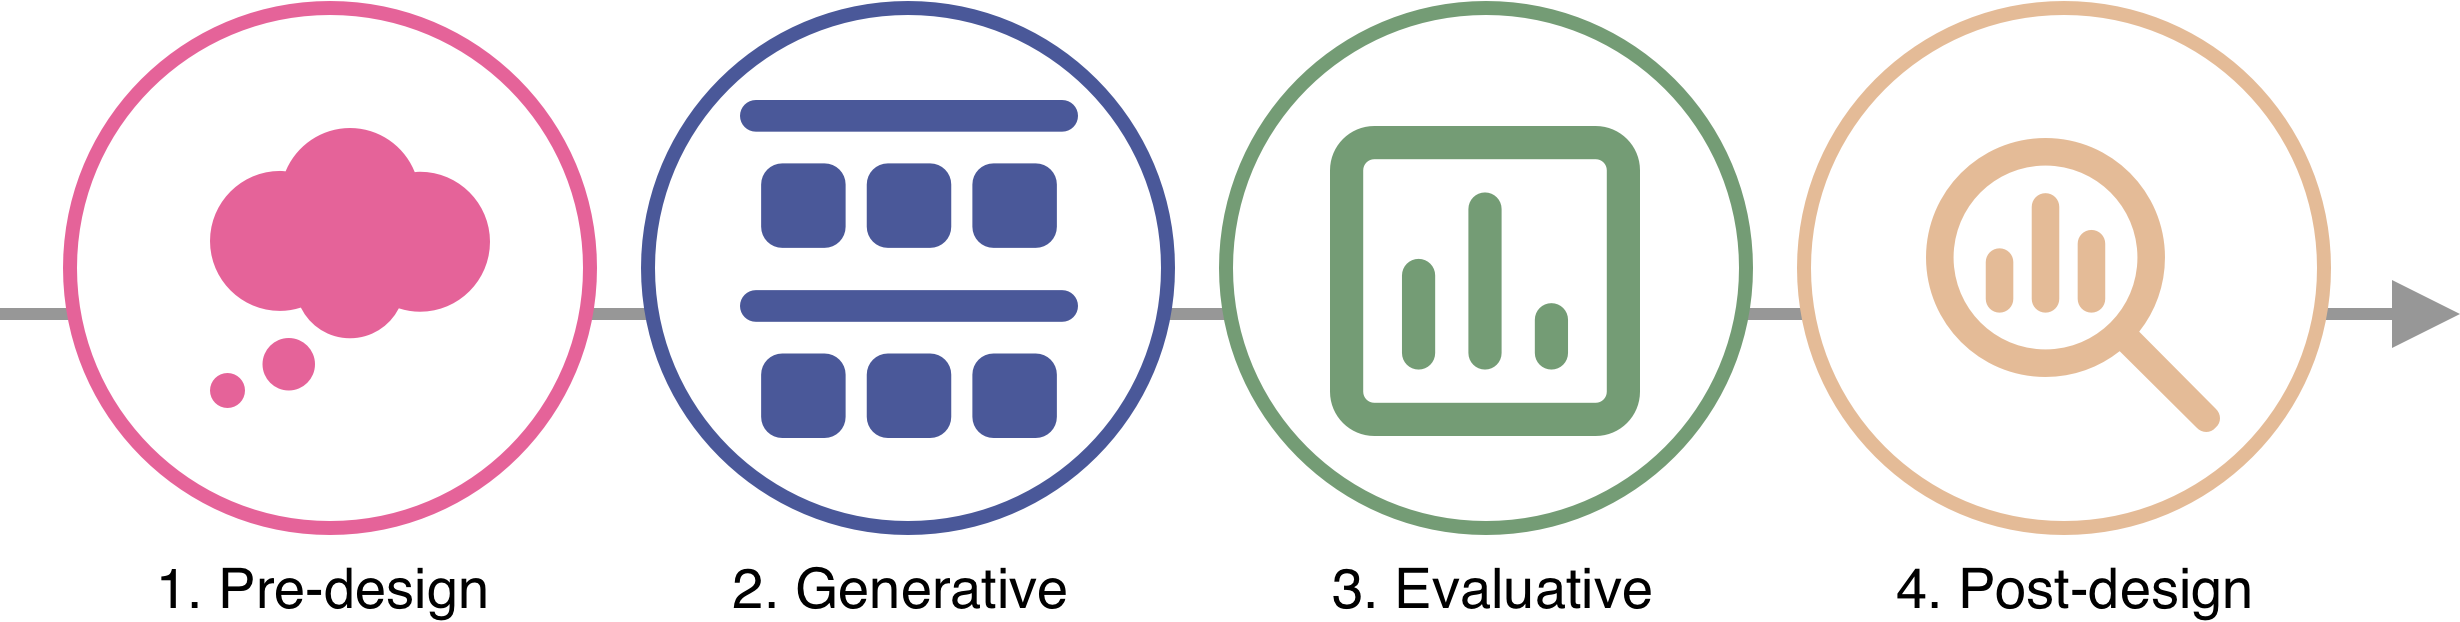
\includegraphics[width=0.8\linewidth]{Images/ChapterTwo/PhasesOfTech.png}
    \caption{Four phases of tech development \citep{suijkerbuijk_active_2019}}
    \label{fig:PhasesOfTech}
\end{figure}
In a recent systematic review of developing supportive technologies for and with people with dementia, \cite{suijkerbuijk_active_2019} categorise technology development into four phases: pre-design, generative, evaluative, and post-design (seen in fig \ref{fig:PhasesOfTech}). In this subsection, I dive into a series of dementia-HCI studies that involve people with dementia in the different stages of development. This sub-section aims to focus on the type of people with dementia who are included (or instead excluded), alongside the type of methods and approaches researchers adopt to involve the voices of people with dementia.

\subsubsection{Pre-design}
\label{BL:Pre-Design}
This literature review began by outlining the different ways HCI researchers have adapted participatory approaches to involve and represent people with dementia in the different phases of technology development. 

\section{Drawing from work outside dementia-HCI space}
\label{BL:Outside-HCI}


\section{Missing gaps in dementia-HCI literature}
\label{BL:Missing-gaps}
This literature review began by outlining how HCI researchers have adapted participatory approaches to involve and represent people with dementia in the different phases of technology development. This final section outlines four gaps of literature that explore the social and political structures that enable (or instead disable) those with dementia to participate and be recognised for their meaningful contributions. 

\subsection{Ethical practice in dementia-HCI}
\label{BL:gap:Ethics}
Participatory and co-design projects have innovated methodological approaches to design, which are necessary to support people with dementia to engage meaningfully in the co-design process. The literature illustrates ways to engage in longer-term projects, work with the family ecology of care, and navigate gate-keeping within institutions. This includes: treating the person with dementia as an individual in context; including the person with dementia in research processes that are explicitly aiming to improve their quality of life; acknowledging that dementia is a complex experience that often also includes social complexity, ageing and multi-morbidities, which require attuning to in design and research responses. It can be argued that these design decisions offer particular ethical stances that appear essential to both the success of HCI projects in this context and ensure the researcher-participant relationship is navigated with mutual respect and care. However, in contrast to the breadth of literature outside of HCI that reflects and demonstrates the relational complexities seen in the everyday interactions of working with people with dementia, dementia-HCI has yet to make these ethical processes more visible.

While dementia-HCI researchers can learn a lot from non-HCI literature on dementia, introducing technology brings additional complexities concerning privacy and data storage; health and educational support; technology longevity, and technology responsibility. Additionally, gatekeeping and consent issues described in the literature need further consideration regarding the influence of ERBs that uphold our work. Pachana et al. further highlight that committees may be \textit{"subject to the same biases and stereotypes present in the general population"}. ERBs unaware of such biases may focus on the aims of protection instead of the approval of research that attends to topics such as agency and ensures meaningful participation. Further complexity arises since ERB decisions vary even within the same country or region \citep{edwards_research_2004}. This is because the decisions and reasoning's are made at a university level and influenced by cultural and local norms and customs. Thus, the disciplinary changes in working with populations such as dementia are not necessarily matched at the level of those who make decisions about what research is and is not allowed when carrying out participatory work with participants who are considered 'vulnerable'.

These challenges have been navigated and discussed in detail through ACM Town Halls and conference workshops. Researchers have been invited to reflect and consider the ethical challenges they face within this space. While recent work in HCI has begun to examine the role of ethics in HCI research - particularly studies that work within sensitive settings, there is a need to come together as a community of practice to identify institutional and relational ethical challenges. In light of this, examining the ethical complexities faced in dementia-HCI work might provide valuable insights into ways to ensure meaningful and engaged research with marginalised groups is central to the design of technologies and systems.


\subsection{Representation of technology and dementia through public engagement}
\label{BL:gap:engagement}
Over the years, people with dementia have shown a growing interest in raising general public awareness about dementia by participating in panels, workshops, blogs and presentations. Innes et al. interviewed six people with dementia who are part of a Dementia Associate Panel (DAP), highlighting how empowering and affirming people with dementia felt when facilitating and educating people on dementia. The study participants continue to describe the benefits of such involvement in public awareness as it promotes a broader perspective of dementia and improvements in dementia support and services.

Within HCI, design and development domains, hackathons have become a popular approach for researchers and organisations to bring together the public to develop new paths to research, ideate, and test software or products. Typically, hackathons have been organised and sponsored by businesses or universities to allow undergraduates to gain experience and practice new skills and potentially build connections between the attendee and organisation recruiters or employees. Hackathons are often coupled with rewards and prize money for the winning team as an enticement to spend time building a demo and/or presentation [49]. Hackathons have also been adopted as opportunities for co-operative makerspaces focusing on health and other community-based issues: for example, hackathons for women’s health [73], and self-harm [5] have offered key insights into how interdisciplinary teams can come together to shape innovative technical responses to complex topics and wicked problems. 

One challenge lies in how we engage such sensitive topics in HCI while encouraging public engagement and facilitating opportunities for collaborative learning and awareness around the topic of interest. While it takes time for researchers to become aware of the sensitivities required for working with such a population, hackathon formats expect the same sensitivities to develop quickly – usually at the weekend. Therefore, it is not surprising that prior work has indicated that some design outputs may be unsuitable or feed into stigmatising ideas of the group or topic at the centre of the design event [89]. Prior work has considered ways to sensitise attendees on the event's topic through presentations, workshops [43], and inspiration packs [5] to upskill participants who may hold outdated or stereotypical attitudes. Given the potential challenges of such public design events, it might be worth considering how representation and attitudes on dementia may be presented in more technical public design events. Further, with people with dementia engaging in public awareness through sharing experiences, facilitation, and presentations, how might design events be structured to support these sensitive conversations better.


\subsection{Promoting learning around dementia and technology}
\label{BL:gap:Learning}
As described in the literature, to support to help foster empathy with, and understanding of, a person with dementia's experience, there has been a push from dementia activists toward using online interactions and bespoke forums and Twitter to raise awareness and further challenge the stigma surrounding dementia [89]. Likewise, Lazar and Dixon's work on dementia activism shares insights into people with dementia proactively coming together online to raise awareness and challenge stereotypes and stigma of current portrayals of living with dementia [53]. This work highlights the online work of a committed group of people with dementia, curating and publishing their experiences, personal views, and providing opportunities for dialogical interactions to happen. However, understanding how those making design decisions on behalf of people with dementia remains sparse. 

Much research in HCI has been devoted to the development of toolkits and other creativity support mechanisms, which have variously been used to support design research, creativity, and technological development and implementation [14,56]. Ledo et al. write that toolkits within HCI provide: a) simplifying and fast-track creation, b) assistance in problem-solving processes, c) help to engage new audiences d) help to adapt tools within users workflows and e) support replication to enable scaling [56]. Peter et al. suggest tools be more "consciously culturally-tailored" (pg.20) [73]. This may require involving audiences in the creation and customisation of the tool. Similarly attending to the practical use of such kits, in a recent review of open-source fairness toolkits, Lee and Singh raise a valuable concern, stating creators of such toolkits should “remain vigilant to ensure their adoption is aligned to the over-arching goal: to ensure our algorithms reflect our ethical values of non-discrimination of fairness” (pg.12) [57]. In cases like these, the provision of tools that may be freely used and reshaped by a user community requires further thought about the roles of moderation or expertise, particularly when toolkits may be intended for use or application in marginalised settings. This open-source framing also, interestingly, opens up the possibility that toolkits might move from being static resources (even so far as being printed, boxed and shipped), to being something that evolves and develops over time (a fluid and unfinalisable design tool).

In reviewing the above, we see that many of toolkits have been developed in response to a given problem or design challenge - whether that has been engagement with a particular community, or to provide insight and knowledge on a complex or novel topic. Prior work has highlighted that the content of such toolkits requires careful consideration, and often a set of expert curators to ensure content is ethical and sensitively designed. However, returning to our dementia literature, such work involving people with dementia requires adaptability to ensure inclusive and meaningful engagement. Furthermore, while there are many different types of toolkits that we look to for inspiration for applications within dementia, we must ensure that the toolkits will adapt and fit into the user’s workflow. In turn, this raises the question of what sorts of toolkit interactions we should provide to designers and developers that allow them to design with people with dementia collaboratively.


\subsection{Attending to mutual collaborative relationships}
\label{BL:gap:relationships}
Fostering independence is central in person-centred approaches, where the person's individuality and abilities are valued. Leverton et al. describe how homecare workers use the person with dementia's identity, wishes, and extensive knowledge about the person to support independence by offering meaningful choices and involvement in decision-making. The independency for making decisions is an integral aspect of citizenship - one that has been examined within disability research and within dementia (Meissner et al., 2017; Samsi and Manthorpe, 2013). However, as dementia is a progressive condition, the change and decline pose challenges to the person with dementia's ability to make decisions. While it is not uncommon for a partner to take it upon themselves to assist or take over the individual's roles within the family, several vital decisions must be carefully considered, such as care planning, care-home placement and eventually - end of life (Fetherstonhaugh et al., 2017).

Fetherstonhaugh et al. (2013) highlight the importance for people with dementia to be involved in decisions that require the care partner to learn how to enable those decision-making processes best. For instance, one participant describes "maintaining close family relationships and trusting friendships" as a way to feel central to the decisions through being acknowledged and consulted. The findings illustrate this as essential in even the minor day-to-day interactions such as taking the bins out, choices for dinner, and day-out activities. Attending to more interdependent and support strategies requires careful consideration towards care partners, knowing the balance between subtle support versus taking over.

Moreover, despite the benefits of supporting the decision-making processes, this can cause a burden for both parties. This is further complicated when the literature demonstrates the need for people with dementia to shared their lived experiences and push for societal change. Johnson et al. (2019). draw attention to the strain and potential "burdening" that this can cause, as people with dementia already often feel as though they need to support others living with the condition and actively challenge misconceptions and stereotypes that the public may hold. This raises interesting challenges about how to ethically engage this community in design processes without overburdening their participation. With this in mind, HCI research needs to examine the ways participation and technology may support the involvement of different voices from the ecology of care while ensuring the person with dementia is well represented and involved in the design making process. 

\section{Summary}
\label{BL:summary}
This review has detailed dementia literature regarding how we represent the experiences of people with dementia and involve them in participatory work. The literature review started with a discussion on the ongoing shift from a bio-medical approach to a more person-centred approach that has been adapted and adopted by the HCI community. Through this discussion, I have highlighted the breadth of work done in HCI that emphasises the need for relationship building, working within ecologies of care, and engaging with participants' creativity. From here, I broaden the literature review to consider dementia literature outside the HCI space. This section examines various ethical considerations for including later stages of dementia, consent and navigating gatekeeping within institutions and organisations. Additionally, to explore the missing gaps in dementia-HCI, I introduce literature concerning the public perception of dementia that describes how HCI work might benefit from such public-facing engagement to support the collaboration of designing technology with people with dementia.

The final section outlines four avenues of investigation for this thesis that orients toward a more critical perspective of dementia. These avenues are not intended to be exhaustive but rather to move towards a multidimensional understanding of dementia and question the adapting roles and situations people with dementia may have within their relationships. To conclude this chapter, it is worthwhile to revisit the research questions in retrospect to the missing gaps found in the literature review:


% Please add the following required packages to your document preamble:
% \usepackage[normalem]{ulem}
% \useunder{\uline}{\ul}{}
\begin{table*}[htp]
\caption{Research questions in regards to the background literature}
\label{BL:RQ}
\begin{tabularx}{\textwidth}{@{} Y|Y @{}}
\textbf{Research question} & \textbf{Areas to explore from literature review}  \\ \hline
How can we use participatory design approaches to provide meaningful and engaging experiences for people with dementia? & Participatory approaches must be co-created with people with dementia and their care partners to improve engagement and inclusion.  \\ \hline
What are the ethical implications for people with dementia to participate in HCI research? & Outside HCI, dementia researchers have built a breadth of information on the ethical complexities of working and representing people with dementia. While the literature review highlights a handful of dementia-HCI papers that reflect on the ethical challenges, there is a gap in the literature to understand the complexities from an HCI perspective.
  \\ \hline
What are the competing interests and expectations to support meaningful dialogue in dementia design research when involving multiple stakeholders - such as people with dementia, developers, designers and researchers? & Lack of involvement of stakeholders who are part of the design process  \\ \hline
\end{tabularx}
\end{table*}


In the next chapter, I describe the methodologies used for this research which examines the role of participatory design approaches to understand the relationships between people with dementia and diverse stakeholders.
